\chapter{Sketching in 3D}

In a typical 2-D sketching application on a graphical tablet, a user draws on a two dimensional plane that mirrors the surface of the input device.
However, in a 3-D sketching application, the user draws on arbitrary three dimensional planes and surfaces.
The most basic example is a simple plane: a user can orient a plane in three dimensional space, and the draw on the tablet.
The strokes on the tablet are then projected onto the plane, thereby creating a 3-D stroke.

The goal is to be able to perform real-time 3D sketching.
We assume that our model environment has been "polygonalized" into triangles.
The constraint is that we need to draw on the image plane with the true perspective image as seen from the observer's position.
Using a perspective image, as opposed to an orthographic image, would give the best understanding of the drawing environment, allowing us to mimic drawing in 3D space.

The difficulty is achieving this at interactive rates, at least as fast as a person draws; roughly 30 frames per second.
This is hard!
We rely on techniques implemented in rendering algorithms, specifically the ray casting methods utilized in ray tracing.
To obtain the speed, it is necessary to reduce the large number (N) of ray-triangle intersections for complex environments. Note that N is large due to the decomposition into many small triangles.
We utilize a spatial tree data-structure containing a hierarchical bounding-box scheme to reduce the computation time. We have been able to achieve this acceleration as shown in Chapter 7. 

In this chapter we provide detailed definitions of:
\begin{itemize}
\item The ray casting approach
\item The method for ray-triangle intersections
\item The hierarchical box and tree data structures:
\item The heuristic Surface Area subdivision
\end{itemize}  
We use all of the above to efficiently project two dimensional user input onto a three dimensional sketching environment.

\begin{figure}
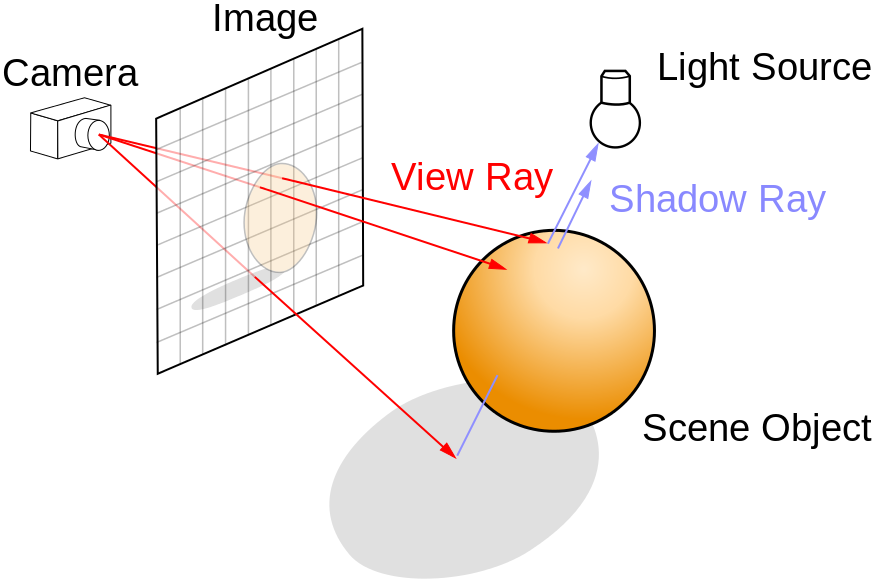
\includegraphics[width=0.9\linewidth]{raytracediagram}
\caption{Ray Tracing in Computer Graphics}
\end{figure} 
\begin{figure}
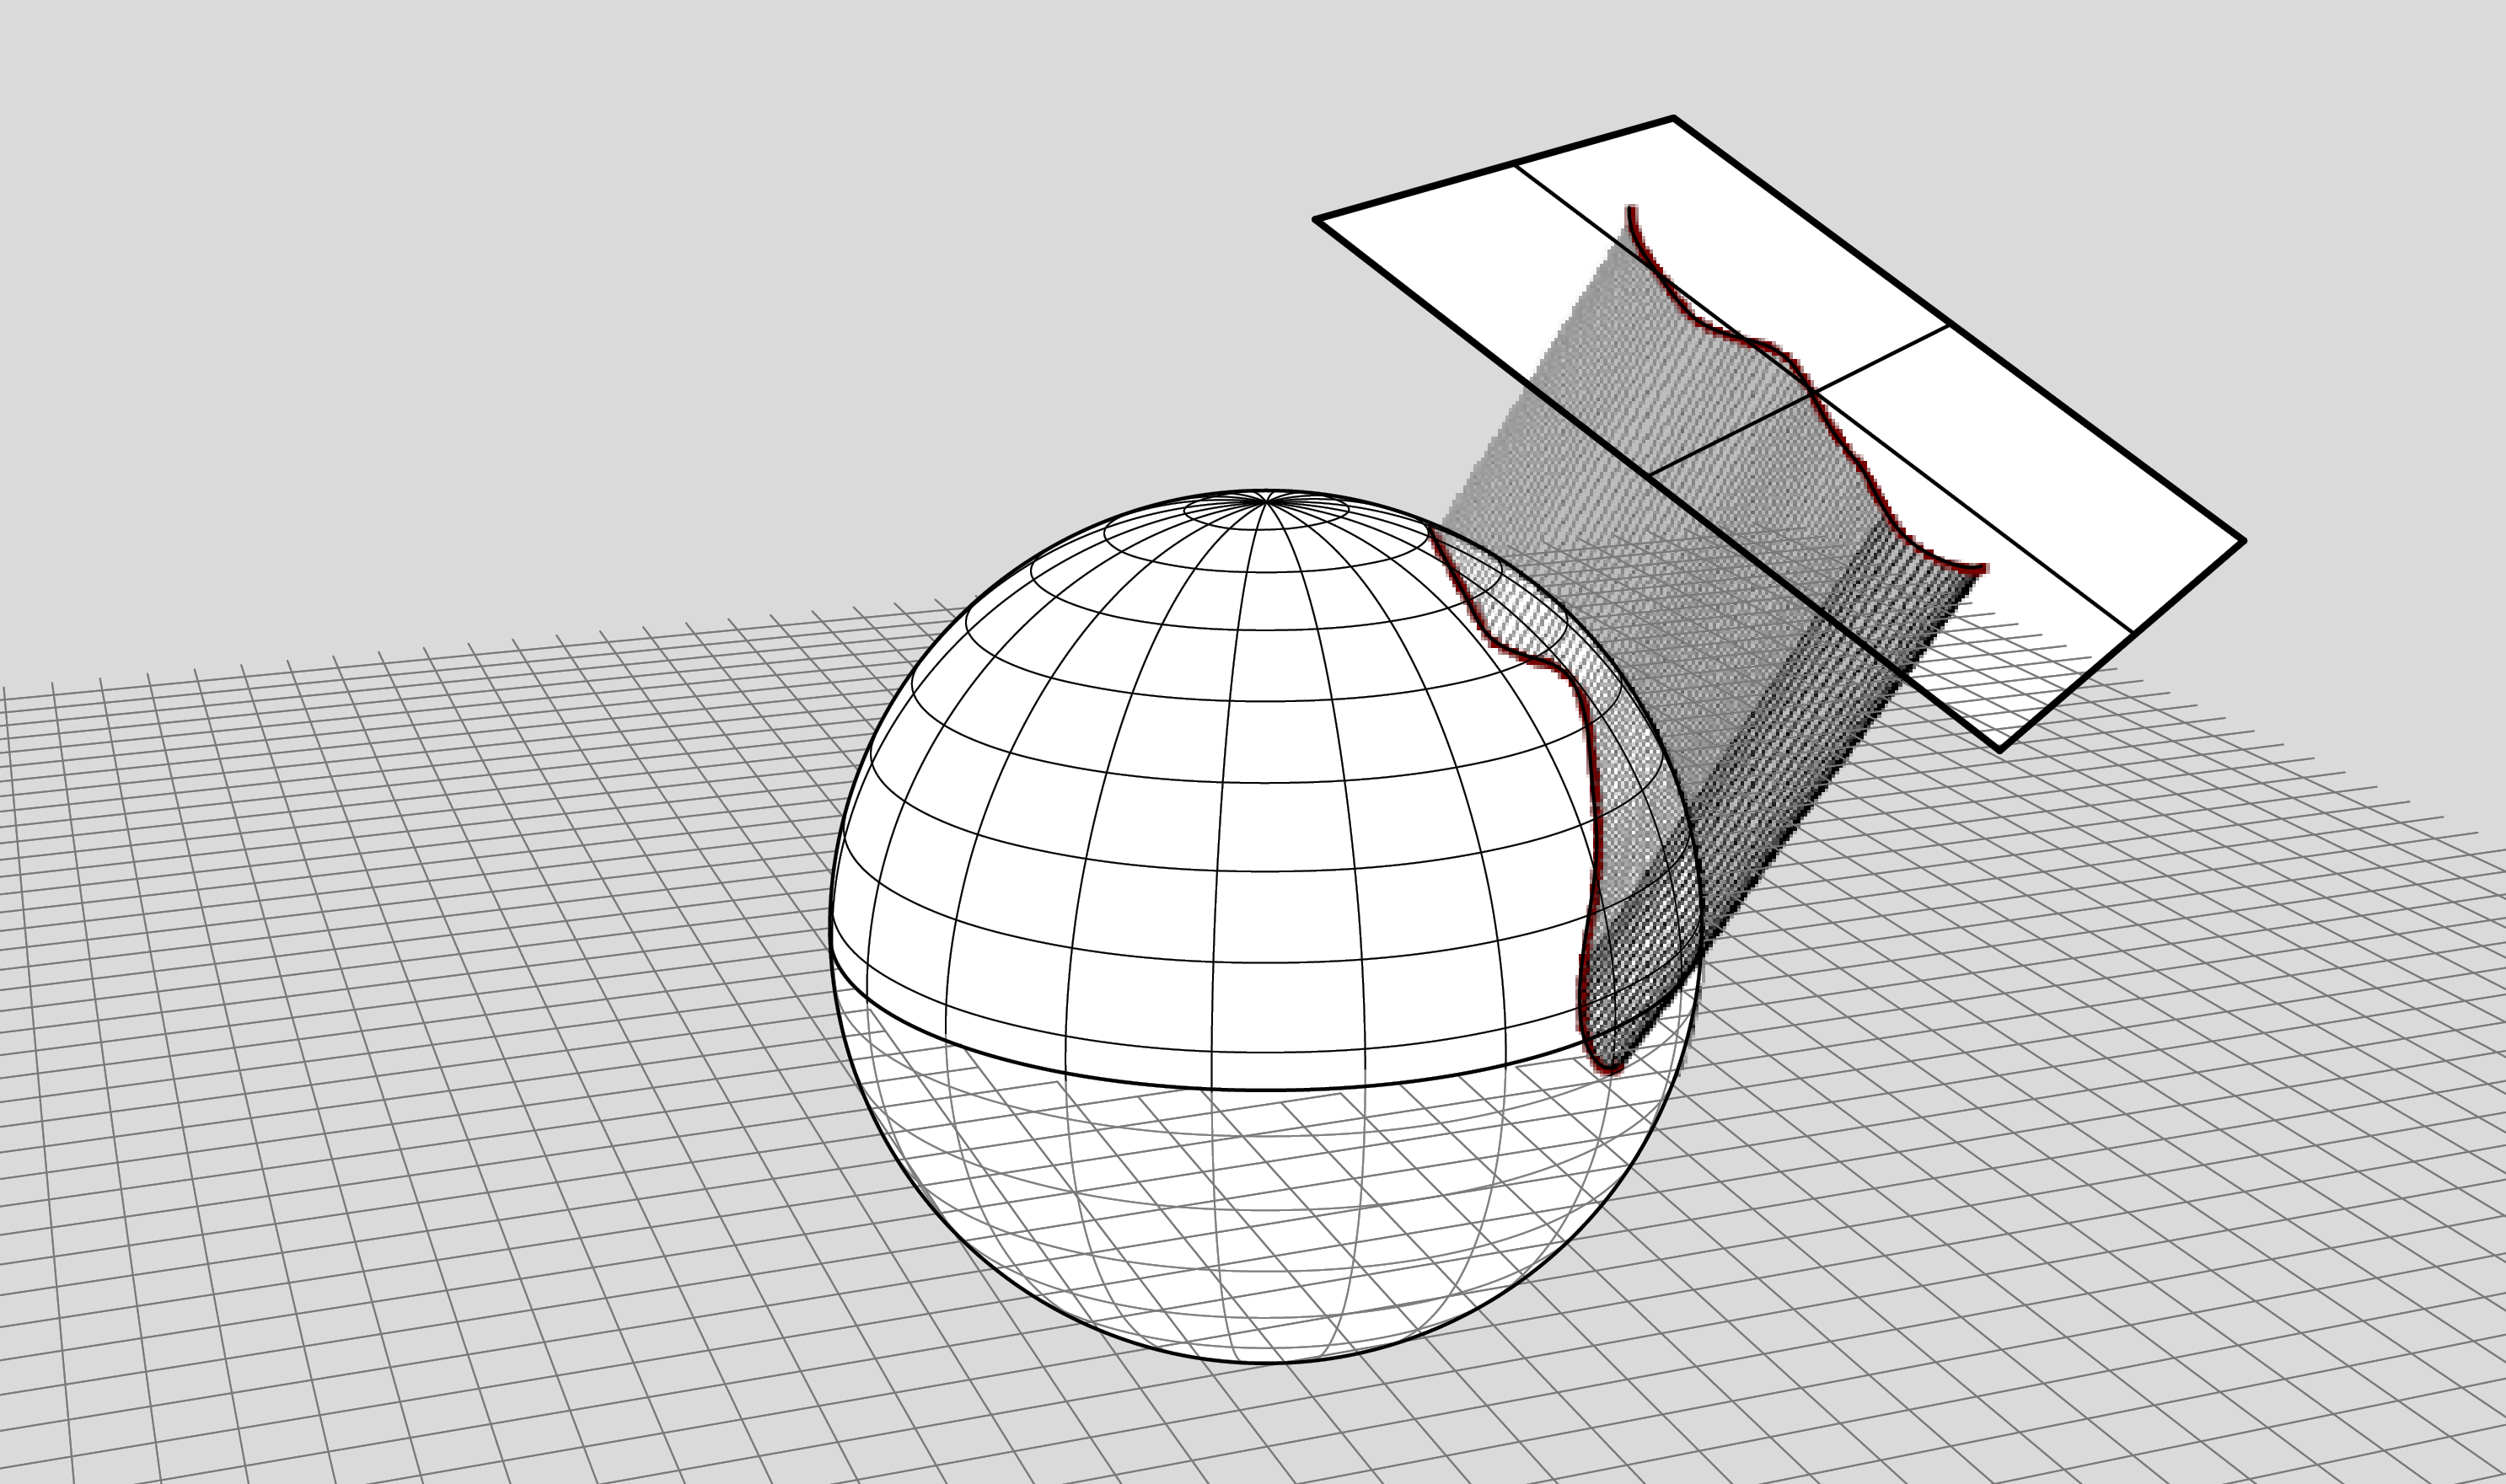
\includegraphics[width=0.9\linewidth]{sketchproj}
\caption[Projecting a Stroke onto the Sketching Surface]{When a user creates a stroke on the screen, the resulting curve is projected onto the sketching surface.}
\end{figure} 

\section{Ray Casting}

Ray casting is the use of rays, a line with an endpoint and a direction, to test for intersections with surface geometry.
These computations are the fundamentals of ray tracing computer graphics algorithms, used to solve a variety of problems.

Ray casting is commonly used for object selection in interactive 3-D applications.
A pointing device provides user input on pixel $(i,j)$, and the "picked" object is whatever is "seen" though the pixel.
Using ray casting, a ray is created and sent in the virtual viewing direction.
The origin of the ray is the position of the camera in the virtual environment, and the direction of the ray is based on the location of the user input.
This is further explained in Section~\ref{sec:raygen}.
If the ray intersects with a surface, that surface is used as the drawing plane.
We can use a similar approach to project our strokes from the screen onto the surfaces of objects.
The ray casting algorithm is utilized as follows:
\begin{enumerate}
\item The user draws a stroke on a 2-D plane, giving a set of sample points
\item An imaginary plane is created in the virtual space representing the image plane.
\item Rays are cast into the three dimensional scene from the imaginary plane based on the sample positions.
\item The intersections with the scene geometry represent the new 3-D positions of the stroke.
\end{enumerate}
Once we intersect all of the sample points with the scene geometry, we can use the spline techniques described in the previous chapter to create a 3-D curve approximating the appearance of the projected 2D stroke.

\subsection{Generating the Ray}
\label{sec:raygen}

OpenGL uses a projection matrix to project the 3D scene to the 2D computer monitor.
First, the matrix transforms points from view space to clip space, the space that defines whether points are visible to the user.
Then the matrix transforms these points to normalized device coordinates (NDC), which causes any visible point to be contained in a box with lower bound (-1,-1,-1) and upper bound (1,1,1). (Figure~\ref{fig:projmatrix})
We want to create rays that match this behavior of OpenGL perfectly, otherwise the user will not be able to draw properly on the surfaces of objects.
The easiest way to accomplish this is to invert the calculations OpenGL uses in order to calculate two points in world space that we can use to generate the view ray.

When the user clicks on the screen, we take the screen point and normalize to a point between (-1,-1) and (1,1).
This represents the X-Y position of the screen point in NDC.
We then create two 3D points $p_0$ and $p_1$ with the XY values of the NDC screen point and z values -1 and 1 respectively to represent the upper and lower bounds of the clip space.
By multiplying these two points by the inverse of the view-projection matrix, we can obtain two points in world space (Figure~\ref{fig:raygen}). 
$p_0$, the point with original z value -1, is the origin of the ray, and the ray direction is equal to $p_1 - p_0$.

\begin{figure}
\label{fig:projmatrix}
\fbox{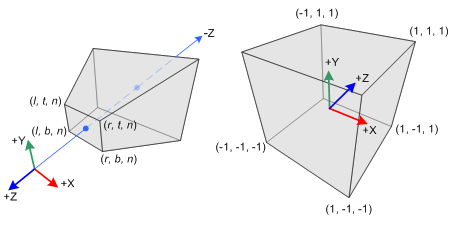
\includegraphics[width=0.98\textwidth]{proj}}
\caption[Clip space and NDC space]{First, the projection matrix transforms points from view space to clip space, the space that defines whether points are visible to the user. Then the matrix transforms these points to normalized device coordinates (NDC), which causes any visible point to be contained in a box with lower bound (-1,-1,-1) and upper bound (1,1,1).}
\end{figure}

\begin{figure}
\label{fig:raygen}
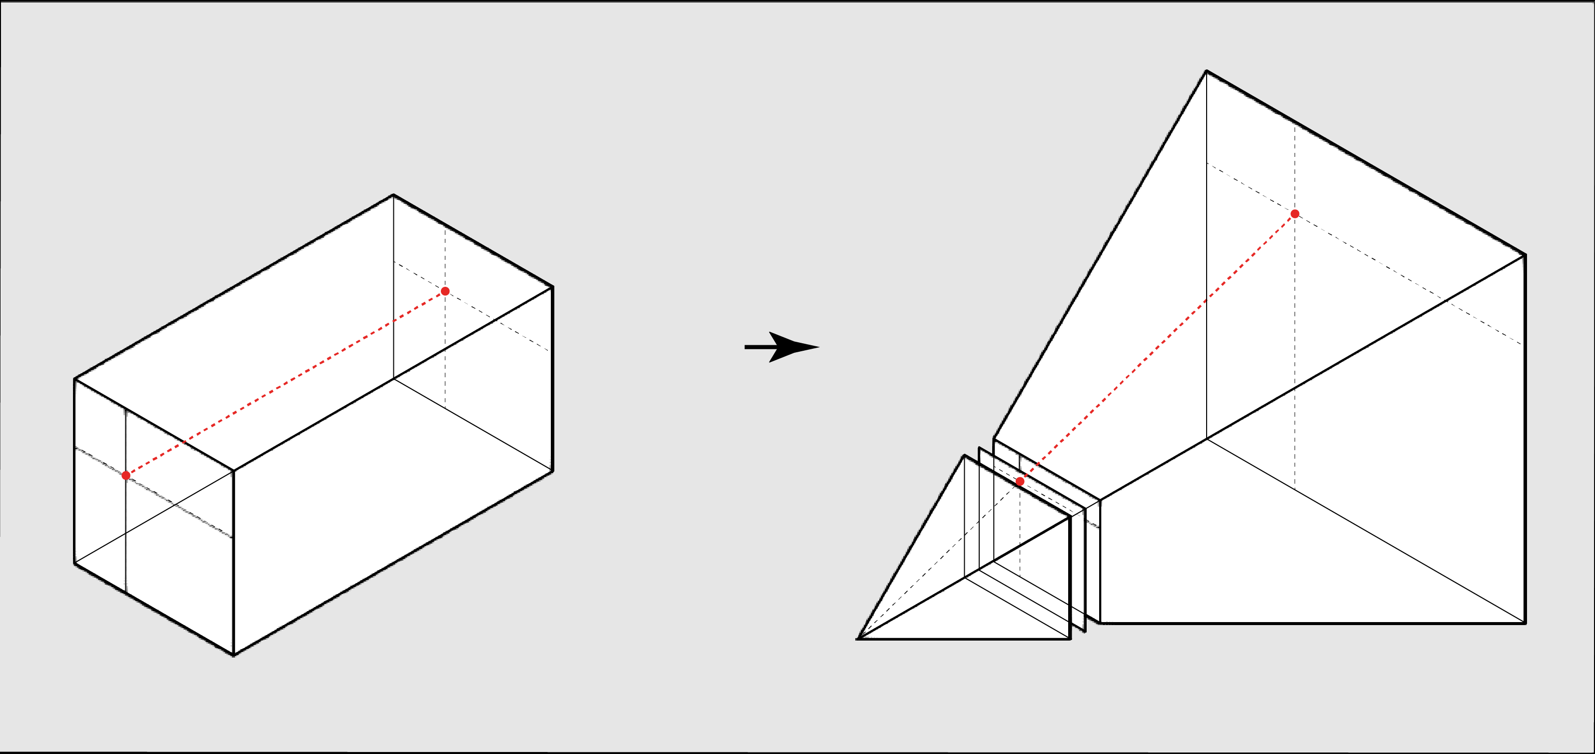
\includegraphics[width=0.98\textwidth]{raygen}
\caption[Generating the Ray]{Using a known point on a 2D screen, we can create a ray in NDC space using the xy point and the z bounds of the space (-1 and 1). Transforming these two points from NDC space to world spaces gives us a line segment that represents what the pixel "sees" in the environment.}

\end{figure}


\subsection{Ray-Triangle Intersection}

Given a ray $\mathbf{e} + t\mathbf{d}$, where $\mathbf{e}$ is the origin of the ray and $\mathbf{d}$ is the ray direction, we want to find the first intersection with any object where $t > 0$.
In this section, the intersection with the most basic computer graphics primitive, the triangle, is discussed.
The use of triangles is prevalent for two primary reasons.
The first is that in order to compute the actual ray-polygon intersection point, one must ensure that it lies within the boundaries of the polygon.
By using triangles, one avoids the computational cost required for re-entrant polygons (polygons with interior angles greater than 180 degrees).
This simplifies the algorithm and allows for hardware implementations.
The second reason is that all surfaces, including spheres or arbitrary parametric surfaces, can be easily approximated using triangles.
Thus, being able to rapidly intersect triangles will allow 3D sketching on any object used for the application.

To demonstrate the algorithm utilized, we will intersect a ray with a parametric plane that contains the triangle.
Once intersected, we use barycentric coordinates to check if the intersection point is contained within the boundaries of the triangle. 
Note we could eliminate this check if we want to draw on an infinite intersection plane.

To intersect a ray with a parametric surface, a system of equations is created where the Cartesian coordinates all match:
\begin{align}
x_o + tx_d = f(u,v) \\
y_o + ty_d = g(u,v) \\
z_o + tz_d = h(u,v)
\end{align}
These three equations contain the three unknowns ($t$, $u$, and $v$).
When the parametric surface is a parametric plane, the parametric equation can be written in vector form.
If the vertices of the triangle are $\mathbf{a}$, $\mathbf{b}$, and $\mathbf{c}$, then the intersection occurs when
\begin{align}
\label{eq:raytreq}
\mathbf{e} + t\mathbf{d} = \mathbf{a} + \beta(\mathbf{c}-\mathbf{a}) + \gamma(\mathbf{c}-\mathbf{a}).
\end{align}
$\beta$ and $\gamma$ are two of the three barycentric coordinates of the triangle. 
If $\beta > 0, \gamma > 0,$ and $\beta + \gamma < 1$, then the intersection point lies inside of the triangle; otherwise it hits the plane outside the triangle.
If there are no solutions, then either the triangle is degenerate or the ray is parallel to the parametric plane.

To solve for $t$, $\beta$, and $\gamma$, Equation~\ref{eq:raytreq} is expanded from the vector form to equations for each of the three coordinate planes.
\begin{align}
x_o + tx_d = x_a + \beta(x_b-x_a) + \gamma(x_c-x_a) \\
y_o + ty_d = y_a + \beta(y_b-y_a) + \gamma(y_c-y_a) \\
z_o + tz_d = z_a + \beta(z_b-z_a) + \gamma(z_c-z_a)
\end{align}
This can be rewritten into a standard linear equation of the form $Ax = b$:
\begin{align}
\label{eq:58}
\begin{bmatrix}
x_a - x_b & x_a - x_c & x_d \\
y_a - y_b & y_a - y_c & y_d \\
z_a - z_b & z_a - z_c & z_d
\end{bmatrix}
\begin{bmatrix}
\beta \\ \gamma \\ t
\end{bmatrix}
= \begin{bmatrix}
x_a - x_o \\ y_a - y_o \\ z_a - z_o
\end{bmatrix}
\end{align}
This can be solved using Cramer's rule: given a system of $n$ linear equations for $n$ unknowns, represented as $Ax = b$, where the $n \times n$ matrix $A$ has a nonzero determinant, and the vector $x = (x_1, \ldots, x_n)^\mathrm{T}$ is the column vector of the variables, the system has a unique solution.
This solution is given by
\begin{equation}
x_i = \frac{\det(A_i)}{\det(A)} \qquad i = 1, \ldots, n
\end{equation}
where  $A_i$  is the matrix formed by replacing the $i$-th column of $A$ by the column vector $b$.
Solving gives the solutions:
\begin{align}
\beta = \frac{\begin{vmatrix}
x_a - x_o & x_a - x_c & x_d \\
y_a - y_o & y_a - y_c & y_d \\
z_a - z_o & z_a - z_c & z_d
\end{vmatrix}}{|A|} \\
\gamma = \frac{\begin{vmatrix}
x_a - x_b & x_a - x_o & x_d \\
y_a - y_b & y_a - y_o & y_d \\
z_a - z_b & z_a - z_o & z_d
\end{vmatrix}}{|A|} \\
t = \frac{\begin{vmatrix}
x_a - x_b & x_a - x_c & x_a - x_o \\
y_a - y_b & y_a - y_c & y_a - y_o \\
z_a - z_b & z_a - z_c & z_a - z_o
\end{vmatrix}}{|A|} 
\end{align}
where A is given in Equation~\ref{eq:58}, and $|A|$ denotes the determinant of $A$.

\section{Acceleration Structures}

An acceleration structure must be used in order to give sub-linear time for ray object intersection for complex objects.
In a naive implementation, the ray caster would iterate over all triangles in the scene to check for intersections, giving $O(N)$ performance.
For sufficiently large values of $N$, this would be very slow; thus a "divide and conquer" algorithmic approach is used, creating an ordered data structure to speed up the intersection process.

While many approaches exist, we implement a simple bounding volume hierarchy (BVH) tree \autocite{bvh}.

\subsection{Bounding Boxes}

A bounding box for a point set $S$ in three dimensions is the box with the smallest measure (volume) within which all the points lie.
For this project, we use axis-alligned bounding boxes (AABBs), which are constrained so their edges lie parallel to the Cartesian coordinate axes (Figure~\ref{fig:aabbray}).
A key operation in any intersection acceleration structure is computing the intersection of a ray and a bounding box.
Since we are interested in the actual ray-surface intersection, it is not necessary to calculate where the ray hits the box, only if it is hit at all, as the box itself is not an actual piece of geometry.

One of the fastest current methods for intersecting a ray with an AABB is the slab method \autocite{hypergraph}.
The idea is to treat the bounding box as the space contained inside of $N$ pairs of parallel planes.
For each pair of planes, two pairs of $t$ values, $t_{min}$ and $t_{max}$ are solved for the segment that is between the two planes.
If the largest $t_{min}$ is smaller than the smallest $t_{max}$, then some portion of the ray is contained within all three planes.

\begin{figure}
\label{fig:aabbray}
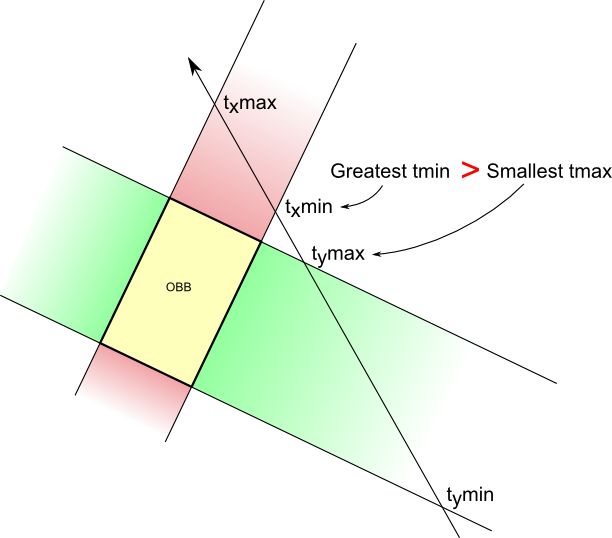
\includegraphics{AABBray}
\caption[AABB Intersection]{For 3D geometries, when checking if a ray intersects a bounding box, the ray is intersected through three pairs of parallel planes defined by the upper and lower bounds of the bounding box. After calculating the pairs of intersection values, the largest of the smaller number of the pairs is compared to the smallest of the larger number. If the largest min is greater than the smallest max, the ray intersects the box. For simplicity, the figure is shown in two dimensions.}
\end{figure}

\subsection{BVH Tree}
 Normally, for intersecting a ray with a scene, one needs to check for the ray's intersection on every piece of geometry.
 To reduce this rather costly computation time, we utilize a bounding volume hierarchy (BVH).
 This is a binary tree data structure superimposed on a set of geometric objects.
 
 There are two main components to the BVH; the nodes, which make up the structure of the tree, and the leaves, which sit at the bottom of the tree.
 The leaves of the tree are sets of geometry of a predetermined maximum size.
 Ideally, the objects contained in the leaves are very spatially close to each other.
 Each node in the tree represents an axis-aligned bounding box in the 3D world.
 The node's shape is defined as the minimum sized bounding box that contains all of the node's children.
 This parental grouping occurs recursively until there is a single bounding volume at the root of the tree. (Figure~\ref{fig:bvhtree})
 
 The algorithm used to construct a BVH can be basically described as follows.
 First, we decide on a cost function that will check the quality of the object division.
 Then, a bounding box is created for the current node.
 At the beginning of the algorithm, this is the root of the tree containing all of our scene geometry.
 We sort along all three axes and find the axis with the least cost according to our chosen cost function.
 We then find a position along the cheapest axis that will be used as the center of subdivision.
 Finally, the objects are divided based on the chosen center into two sub-groups.
 Two child nodes are created from these sub-groups, and the algorithm repeats.
 When a small enough number of objects are in each node, the algorithm terminates.
 
 \begin{figure}
 \includegraphics[width=\textwidth]{bvhtree}
 \caption[BVH Tree]{An example of a Bounding Volume Hierarchy (BVH). At each node, if the contained number of objects is higher than our predetermined maximum (in this example, two), the node branches into two. For simplicity, the figure is shown in two dimensions. \autocite{ray1}}
 \label{fig:bvhtree}
 \end{figure}
 
 
 By using this data structure, we only need to traverse a small portion of the total scene.
 For example, if the ray does not intersect the root bounding box of the scene, we know that the ray does not intersect any of our scene geometry.
 This reduces the computational complexity of a ray intersecting a scene from linear time $O(N)$ to logarithmic time $O(log(N))$.
 
 A good BVH tree has the following properties:
 \begin{itemize}
 \item The nodes in a given sub tree should be close to each other. The lower down the tree, the closer the nodes should be.
 \item Each node in the BVH should be of minimum volume.
 \item The sum of all bounding volumes should be minimized.
 \item The volume of overlap of sibling nodes should be minimized.
 \item The BVH should be balanced with respect to both its node structure and its content. Balancing allows as much of the BVH to be pruned when not traversed.
 \end{itemize}
The quality of a BVH tree is mostly determined by how the objects are subdivided between child nodes.
One of most commonly used splitting heuristics is the Surface Area Heuristic (SAH) \autocite{sah}.
The idea behind SAH is to balance both the number of objects contained in a bounding volume while minimizing the surface area of the volume itself.
This is an exceptionally slow heuristic when constructing the tree, but currently provides the fastest solution at runtime.
Thus the construction cost should be considered for use in real time applications.
For our application, we decided to sacrifice the construction costs in order to allow for higher polygonal complexity.

\begin{figure}
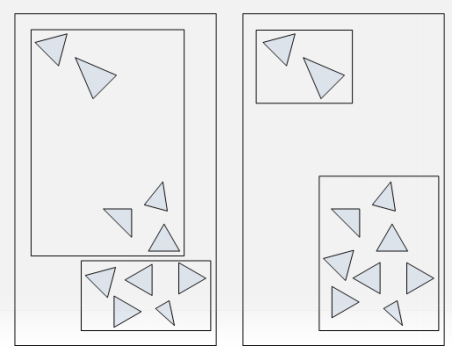
\includegraphics[width=\textwidth]{sahbvh}
\caption[SAH Comparison]{A comparison between the bounding volumes of a node using a naive heuristic(left) and a surface area heuristic (right). Note that for SAH, the total area of the child bounding boxes is much smaller than that of the naive approach. For simplicity, the algorithm is shown in two dimensions.}
\end{figure}

\section{Summary}

Using the algorithms described in this chapter, we have been able to project our sketch strokes from the two dimensional input surface to the three dimensional model environment.
The acceleration structures allow the use of highly complex models with high polygonal counts while maintaining a relatively fast runtime.
Using the above algorithm, we have been able to sketch on complex three dimensional objects at interactive rates.